% Example note for /write-note, made up for illustration. The team (T00: Alex, Sam, Kim), its
% question history, checks table and AI logs are fictional. The physics and the numbers are real:
% they come from fig_phase.example.py in this folder (Haldane model, 1.4 s on a laptop), and
% provenance.example.md traces each one. Built with ../scripts/note_check.py --build.
\documentclass[reprint,aps,prl,superscriptaddress,amsmath,amssymb,floatfix]{revtex4-2}
\usepackage{graphicx}
\usepackage{newunicodechar}
\graphicspath{{../figures/}{figures/}{./}}
% Unicode symbols that often appear in text copied from README.md or checks.md
\newunicodechar{′}{\ensuremath{'}}
\newunicodechar{″}{\ensuremath{''}}
\newunicodechar{−}{\ensuremath{-}}
\newunicodechar{±}{\ensuremath{\pm}}
\newunicodechar{×}{\ensuremath{\times}}
\newunicodechar{·}{\ensuremath{\cdot}}
\newunicodechar{≤}{\ensuremath{\leq}}
\newunicodechar{≥}{\ensuremath{\geq}}
\newunicodechar{≈}{\ensuremath{\approx}}
\newunicodechar{≠}{\ensuremath{\neq}}
\newunicodechar{∥}{\ensuremath{\parallel}}
\newunicodechar{⊥}{\ensuremath{\perp}}
\newunicodechar{→}{\ensuremath{\to}}
\newunicodechar{√}{\ensuremath{\surd}}
\newunicodechar{∞}{\ensuremath{\infty}}
\newunicodechar{°}{\ensuremath{^\circ}}
\newunicodechar{₀}{\ensuremath{_0}}\newunicodechar{₁}{\ensuremath{_1}}\newunicodechar{₂}{\ensuremath{_2}}
\newunicodechar{₃}{\ensuremath{_3}}\newunicodechar{₄}{\ensuremath{_4}}\newunicodechar{₅}{\ensuremath{_5}}
\newunicodechar{⁰}{\ensuremath{^0}}\newunicodechar{¹}{\ensuremath{^1}}\newunicodechar{²}{\ensuremath{^2}}
\newunicodechar{³}{\ensuremath{^3}}\newunicodechar{⁻}{\ensuremath{^-}}
\newunicodechar{α}{\ensuremath{\alpha}}\newunicodechar{β}{\ensuremath{\beta}}
\newunicodechar{γ}{\ensuremath{\gamma}}\newunicodechar{δ}{\ensuremath{\delta}}
\newunicodechar{ε}{\ensuremath{\varepsilon}}\newunicodechar{θ}{\ensuremath{\theta}}
\newunicodechar{κ}{\ensuremath{\kappa}}\newunicodechar{λ}{\ensuremath{\lambda}}
\newunicodechar{μ}{\ensuremath{\mu}}\newunicodechar{ν}{\ensuremath{\nu}}
\newunicodechar{π}{\ensuremath{\pi}}\newunicodechar{ρ}{\ensuremath{\rho}}
\newunicodechar{σ}{\ensuremath{\sigma}}\newunicodechar{τ}{\ensuremath{\tau}}
\newunicodechar{φ}{\ensuremath{\phi}}\newunicodechar{χ}{\ensuremath{\chi}}
\newunicodechar{ψ}{\ensuremath{\psi}}\newunicodechar{ω}{\ensuremath{\omega}}
\newunicodechar{Γ}{\ensuremath{\Gamma}}\newunicodechar{Δ}{\ensuremath{\Delta}}
\newunicodechar{Φ}{\ensuremath{\Phi}}\newunicodechar{Ω}{\ensuremath{\Omega}}

\begin{document}

\title{The Haldane Phase Diagram as a Laptop Benchmark, Boundary within One Grid Step}

\author{Alex}
\author{Sam}
\author{Kim}
\affiliation{Department of Physics, Example University}
\collaboration{Team T00, Many-Body Intelligence 2026}
\date{30 November 2026}

\begin{abstract}
We set out to ask how third-neighbour hopping changes the Chern-number phase diagram of the
Haldane model, and narrowed the day to its benchmark. A gauge-free lattice calculation on a laptop
reproduces the analytic phase diagram to within one grid step, the gap closes at a single valley
on each boundary, and the result is unchanged on a coarser momentum mesh. The extension to
third-neighbour hopping is set up but not yet checked.
\end{abstract}

\maketitle

\textit{1. Title, team ID, members.}---Title above; team T00: Alex, Sam, Kim.

\textit{2. Question history.}---Copied from \texttt{README.md}:
\begin{itemize}\setlength{\itemsep}{0pt}\setlength{\parskip}{0pt}
  \item Q0 (proposal): How does third-neighbour hopping t₃ change the Chern-number phase diagram of the Haldane model?
  \item Q1 (sharpened, end of Scope): Does the Haldane phase diagram survive third-neighbour hopping t₃ ≤ 0.1 t₁ at t₂ = 0.1 t₁, as a function of φ and M/t₂?
  \item Done today means: the t₃ = 0 diagram reproduced and checked as a benchmark, and the boundary shift at one value of t₃.
  \item Expected at the end of the day: the boundary moves outward with t₃, by less than one grid step at t₃ = 0.05 t₁.
  \item Confidence (1–5): 3
  \item Q2 (narrowed, time + reason): At the end of First result, because one t₃ scan takes about 40 minutes: reproduce and check the t₃ = 0 diagram; the t₃ shift moves to ``next''.
  \item Final (as stated in the note): The Haldane phase diagram is reproduced on a laptop within one grid step of the analytic boundary; the shift with t₃ is not yet checked.
\end{itemize}

\textit{3. Approach and methods.}---We use the Haldane model on the honeycomb lattice, with
nearest-neighbour hopping $t_1$, next-nearest-neighbour hopping $t_2e^{\pm i\phi}$ and a sublattice
potential $\pm M$~\cite{Haldane}. The Chern number $C$ of the lower band is computed from the
lattice field strength of Fukui, Hatsugai, and Suzuki~\cite{FHS} on a $24\times24$ mesh of the
Brillouin zone, which avoids choosing a smooth gauge. We fix $t_1=1$ and $t_2=0.1$ and scan 41
values of $\phi\in[-\pi,\pi]$ and 41 values of $M/t_2\in[-6,6]$, in steps of 0.3. The phase
$+\phi$ belongs to next-nearest-neighbour hops that run anticlockwise around a hexagon. One NumPy
script produces every number below in about 1.4~s on a laptop.

\begin{figure}[t]
  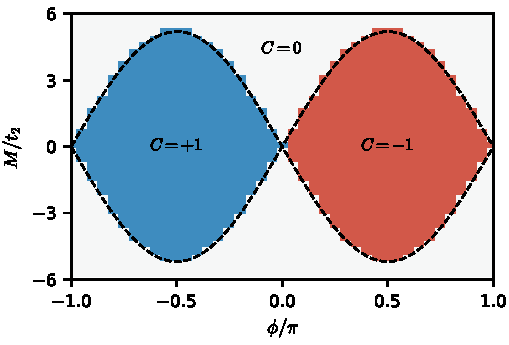
\includegraphics[width=\columnwidth]{phase.pdf}
  \caption{Chern number of the lower band (blue $C=+1$, red $C=-1$, white $C=0$) on a
  $41\times41$ grid; dashed, the analytic boundary $M=\pm3\sqrt3\,t_2\sin\phi$. $t_1=1$, $t_2=0.1$,
  $24\times24$ momentum mesh.}
  \label{fig:1}
\end{figure}

\textit{4. Main result.}---The computed Chern numbers reproduce Haldane's phase diagram:
$C=-\mathrm{sgn}(\sin\phi)$ for $|M|<3\sqrt3\,t_2|\sin\phi|$ and $C=0$ outside, with one of the
1681 grid points off, next to the boundary [Fig.~\ref{fig:1}]. The boundary is where the gap
closes at a Dirac point. At $M=3\sqrt3\,t_2$ and $\phi=\pi/2$ the gap vanishes at one valley (below
$10^{-15}t_1$) and stays at $2.08\,t_1$ at the other, so $C$ changes by one across each boundary.
The sign of $C$ follows from the orientation of the hopping phase and is a convention; its
magnitude and the boundary are not.

The boundary was checked against Haldane's analytic result by a person, and the diagram on a
$12\times12$ mesh agrees at 99.9\% of the points (second AI session). The sign convention was
checked against the paper by a person after a first error, and the gap closing at one valley by a
second AI session (Table~\ref{tab:checks}). Not checked: the shift of the boundary with $t_3$; one
scan was started but not finished in the time available.

\textit{5. Checks table.}---Table~\ref{tab:checks} lists the checks of the results, copied
unchanged from \texttt{checks/checks.md}.

\begin{table*}[t]
  \caption{Checks of the results (copied unchanged from \texttt{checks/checks.md}).}
  \label{tab:checks}
  \begin{ruledtabular}
  \begin{tabular}{p{2.6cm}p{4.0cm}lllp{3.8cm}}
    Result & Check & Method & Done by & Outcome & What changed \\
    \hline
    Phase diagram, t₃ = 0 & Boundary against Haldane's analytic result 3√3 t₂ sin φ & literature & person & holds & nothing \\
    Phase diagram, t₃ = 0 & Same diagram on a 12 × 12 k-mesh & convergence & second-AI & holds & nothing \\
    Chern-number code & Sign of the hopping phase against the paper's convention & re-derivation & person & fails, then holds & Next-nearest-neighbour vectors reordered to run anticlockwise \\
    Gap closing at the boundary & Gap at both valleys at M = 3√3 t₂, φ = π/2 & limiting-case & second-AI & holds & README wording corrected: one valley, not both \\
  \end{tabular}
  \end{ruledtabular}
\end{table*}

\textit{6. How AI was used.}---From the eleven log entries of three people:
\begin{itemize}\setlength{\itemsep}{0pt}
  \item The AI wrote the Chern-number code and the figure script (used after edits) and ran the
  mesh comparison in a separate session.
  \item One AI error mattered: the first code ordered the next-nearest-neighbour vectors
  clockwise, which flipped the sign of every Chern number. A person found it by deriving the
  convention from Haldane's paper by hand.
  \item The AI's literature summary credited the phase boundary to the wrong paper; the team
  corrected it after opening the PDF.
  \item A suggestion to compute the Berry curvature by finite differences was discarded in favour
  of the gauge-free lattice method. The scoping, the narrowing of the question and all checks
  marked ``person'' were done by people.
\end{itemize}

\textit{7. What would come next.}---The question we set out with, how third-neighbour hopping
moves the boundary, is now one parameter away: the same code with $t_3$ added, on a coarser
$21\times21$ grid that takes about ten minutes, checked against the gap closing at the new Dirac
points. A longer project would map where $t_3$ creates new Dirac points and phases with $|C|=2$.

\textit{8. Requested treatment in the joint paper.}---Brief summary.

\textit{Appendix: AI log.}---The log files \texttt{log/P\#\#.md} are attached in the repository as
they are; they do not count toward the two pages.

\begin{thebibliography}{2}
  \bibitem{Haldane} F. D. M. Haldane, Phys. Rev. Lett. \textbf{61}, 2015 (1988),
  doi:10.1103/PhysRevLett.61.2015.
  \bibitem{FHS} T. Fukui, Y. Hatsugai, and H. Suzuki, J. Phys. Soc. Jpn. \textbf{74}, 1674 (2005),
  doi:10.1143/JPSJ.74.1674.
\end{thebibliography}

\end{document}
